%%%%
\section{Poluição do ar em cidades}

A poluição do ar ambiental nas cidades dos países em desenvolvimento
guarda algumas similaridades com as cidades dos países desenvolvidos, pois
ambas possuem fontes poluidoras comuns a meios urbanos, dentre as quais se 
destacam o tráfego de veículos automotivos, as indústrias e a geração de
eletricidade por usina hidrelétrica ou termelétrica.

No entanto, em cidades de países industrializados tardiamente, soma-se a esta 
poluição agravantes decorrentes da má distribuição de 
renda e incapacidade do Estado em atender toda a população nas demandas urbanas 
por infraestrutura. É o caso, por exemplo, da insuficiência de energia para 
realização de atividades cotidianas de transporte, iluminação e alimentação. 
A queima de biomassa para cozimento de alimentos, o uso de querosene para 
iluminação noturna e a frota veicular velha e com tecnologias 
ultrapassadas são alternativas encontradas pelas populações para lidar 
com tal realidade \citep{brauer2012}.

Os fatores supracitados e a urbanização rápida e descontrolada ocorrida na
última década fazem com que cidades da Ásia, África e Oriente 
Médio possuam os maiores níveis de poluição do ar ambiental do mundo 
\citep{brauer2012}. Ainda de acordo com as Nações Unidas \citeyearpar{UN}, 
o crescimento da urbanização nestes países é acompanhado da proliferação de 
favelas e acampamentos nas periferias das cidades, forçando as pessoas a 
fazerem mais uso de veículos, público ou individual, em distâncias e 
tempos longos. 
	
%%%%
\section{África Subsariana}

A África é o terceiro maior continente em extensão, com área territorial 
de 30 milhões de quilômetros quadrados, abrigando 54 países independentes. 
Em 2015, contava com 1,2 bilhões de habitantes, ficando atrás 
apenas da Ásia, que possuía 4,4 bilhões de habitantes no mesmo ano.
 
Em relação ao relevo, destaca-se uma barreira natural formada pelo deserto do 
Saara separando norte e sul, barreira não só geográfica, como social, étnica 
e econômica, pois o sul, conhecido como África Subsariana (SSA), 
conta com os países mais pobres do mundo \citep{UN}. 

Os países da SSA iniciaram nas últimas décadas um intenso processo de urbanização e
industrialização e são os que atualmente possuem a maior taxa de transição no 
mundo da população rural - ainda predominante - para as cidades 
\citep{MONTGOMERY2008}. 
 
Até 2003, nenhuma cidade da SSA possuía sistemas de monitoramento 
sistemático de poluição do ar. Havia somente medidas esporádicas realizadas
por universidades, mas que revelaram concentrações de poluentes altíssimas e 
acima das recomendados pela Organização Mundial de Saúde (OMS) 
\citep{EZZATI2004}.

Segundo \citet{aboh2009} ainda há poucos estudos caracterizando o 
aerossol atmosférico e suas fontes em países africanos, em especial os da SSA; 
entretanto, este número vem crescendo, devido ao fato do aerossol atmosférico 
africano afetar o clima em escala mundial, além dos altos níveis de 
concentrações encontrados em estudos acadêmicos (esporádicos).

Diferentemente dos países industrializados, onde as principais fontes de 
poluição são os setores da indústria e do transporte, nos países da SSA a 
queima de biomassa para preparação de alimentos e a queima de lixo 
doméstico a céu aberto assumem posição destacada, pois são empregadas tanto em 
regiões rurais, quanto urbanas, principalmente em bairros pobres, 
em parte por não disporem de sistema de coleta de lixo frequente ou 
mesmo como forma de evitar o pagamento de serviços de recolha \citep{SMITH2004}.

Resumidamente, os seguintes fatores ampliam as diferenças entre as cidades da 
SSA e as dos países industrializados no que diz respeito a efeitos na 
poluição do ar:
 
\begin{itemize}
\begin{spacing}{1.0}
  \item População predominantemente rural, mas em transição;
  \item Excesso de vias não pavimentadas, mesmo nos centros das cidades;
  \item Alta taxa de crescimento populacional, sem a correspondente melhoria 
        na infraestrutura de serviços públicos;
  \item Emprego de queima de biomassa ou de lixo a céu aberto;
  \item Inexistência de sistemas de monitoramento sistemático e em larga escala
        de parâmetros ambientais, realizados por agências de controle.
\end{spacing}
\end{itemize}

%%%%
\newpage
\section{Gana}

%%%%
\subsection{Aspectos geográficos}

\begin{figure}[H]
  \centering
  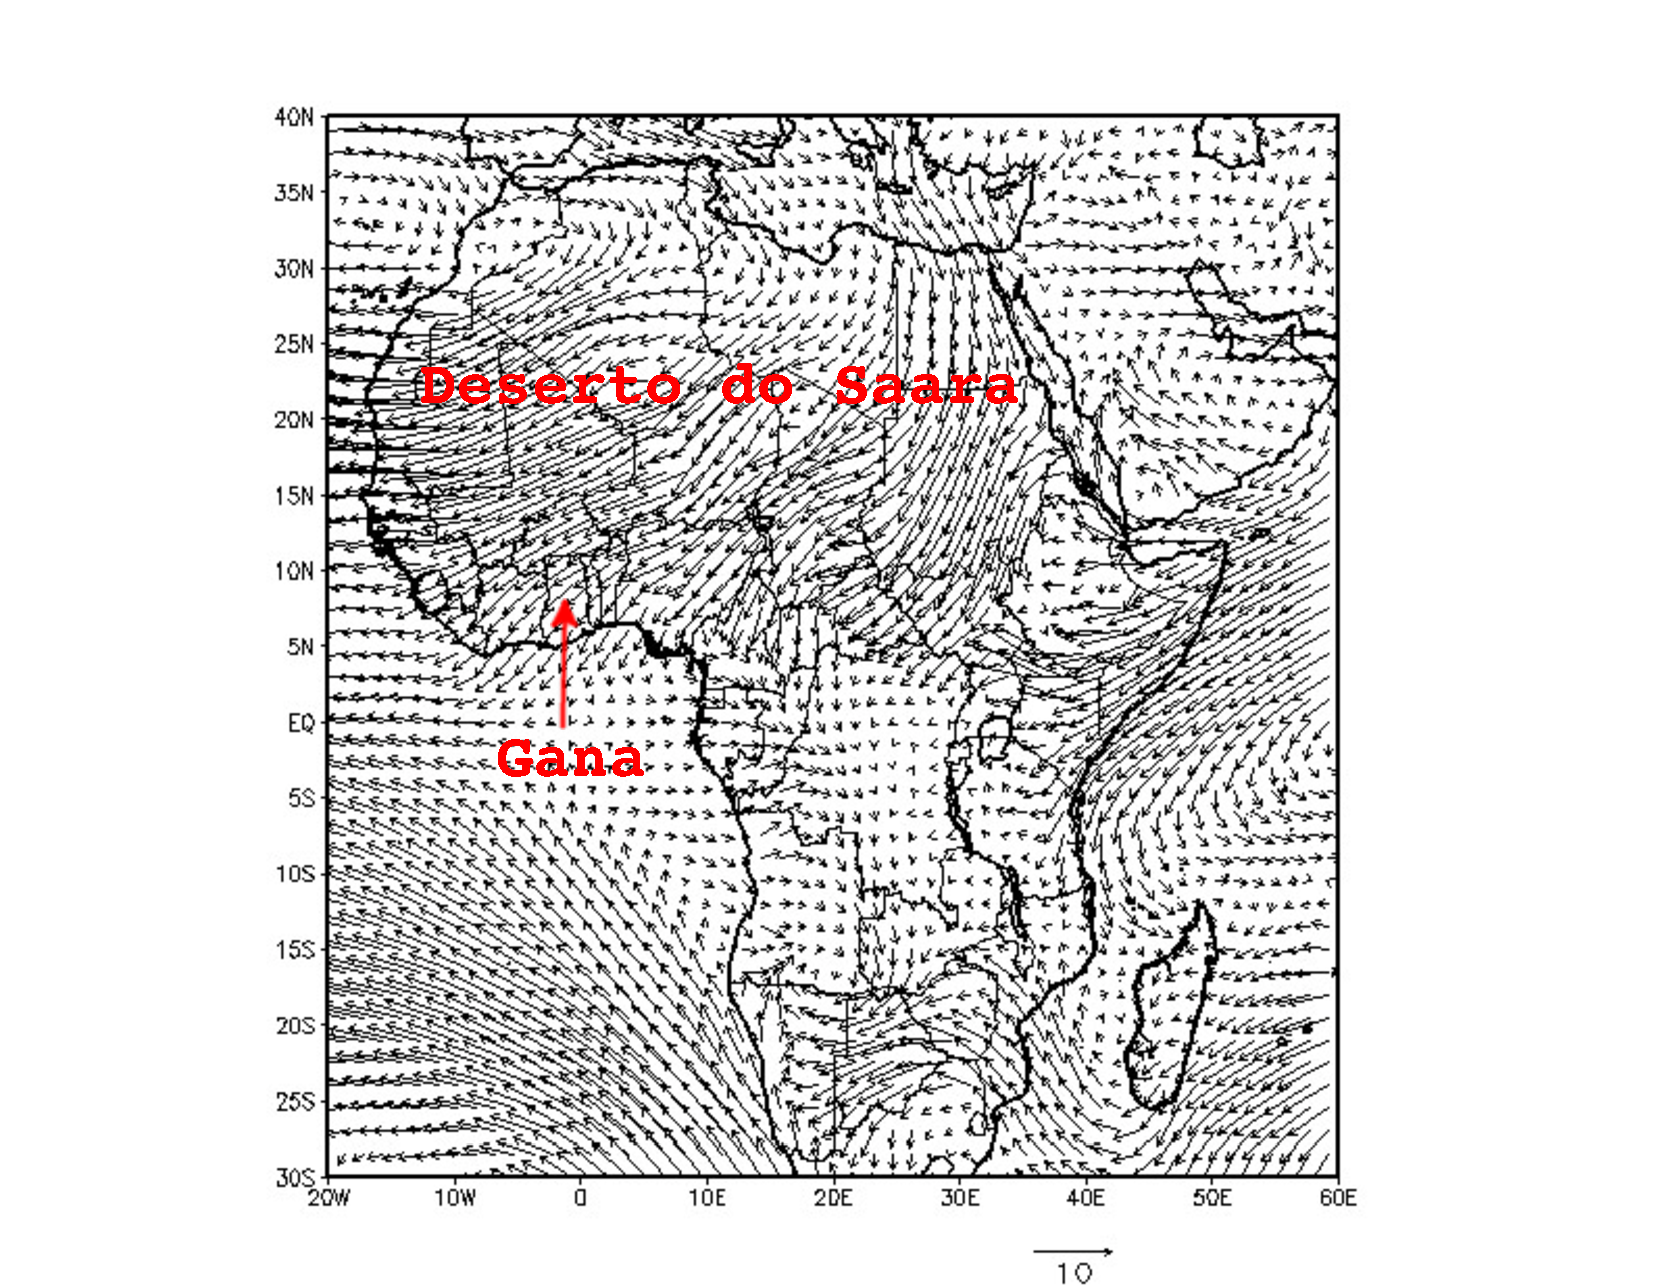
\includegraphics[width=\textwidth]{../inputs/grads/gimp/875hPa/JAN_2008.pdf}
  \caption{Média mensal de direção e intensidade do vento sobre o continente 
           Africano em 875 hPa (aproximadamente 1200 m) em janeiro de 2008.
          \label{fg:ECMWFjan2008}}
\end{figure}

Gana situa-se no continente Africano, na SSA, em torno de 5 graus ao norte 
do Equador e  faz fronteira com Costa do Marfim a oeste, ao norte com Burkina
Faso e a leste com Togo, sendo a costa sul litorânea e voltada para o oceano 
atlântico.
De clima equatorial, possui praticamente duas estações climáticas, 
entre novembro e março, com ar quente e seco, caracterizada pela chegada de
poeira do deserto do Saara, fenômeno conhecido como Harmatão, e a estação 
chuvosa ocorre entre abril e outubro, com maior intensidade de chuvas 
entre abril e julho. 

O mapa da figura \ref{fg:ECMWFjan2008} posiciona Gana e o deserto do Saara, 
ao norte, e ilustra a média mensal da direção e intensidade do vento 
sobre o continente Africano (longitudes -20 à 60 graus e latitudes de -30 à 40 
graus) durante o mês de janeiro de 2008 em altitude em torno dos 1200 metros 
em relação ao solo, usando dados de reanálise disponibilizados pela 
European Centre for Medium-Range Weather Forecasts (ECMWF). 

O deserto do Saara é considerado a maior fonte de poeira do mundo segundo 
\citet{breuning2005} e \citet{prospero2002}, sendo o Harmatão um fenômeno que 
ao espalhar essa poeira por locais onde passa, como Chade, Nigéria, 
República do Níger, Gana, entre outros, influência o clima e a poluição do ar 
local desses países.

Análises de modelos receptores 
realizadas tanto neste trabalho quanto em \citet{aboh2009}, \citet{dionisio2010b}, 
\citet{zhou2011}, \citet{ofosu2012} e \citet{rooney2012} mostram que ele 
representa a principal 
fonte de partículas de Gana, tanto na fração fina $MP_{2,5}$, quanto na grossa 
$MP_{2,5-10}$.

%%%%
%\newpage
\subsection{Indicadores sociais}

Os últimos censos demográficos em Gana foram realizados em 2000 e 2010 
e publicados em \citeyear{ghanacensus2003} e \citeyear{ghanacensus2013}, 
respectivamente. O relatório final, tabelas e gráficos estão disponíveis
publicamente no portal de dados abertos do Governo Federal de Gana 
\citep{opendataghana}.

\begin{wrapfigure}{l}{8cm}
  \centering
  \includegraphics[width=0.5\textwidth]{../outputs/piramide_etaria.pdf}
  \caption{Pirâmide etária, Gana 2010. \citep{ghanacensus2013} 
           \label{fig:piramedegana}}
\end{wrapfigure}

Em uma década, a população no país teve aumento de 30\%, saindo de 18,9 milhões em 
2000 para 24,7 milhões de habitantes em 2010. Em 2010, a expectativa média de 
vida foi de 60,2 e 63,4 anos para homens e mulheres, respectivamente.
População jovem, como indica a pirâmide etária da figura \ref{fig:piramedegana}.

Em 2010, 49\% da população habitava o meio rural e 51\% no meio urbano, 
sendo que as mulheres representam 51,2\% da população total.

A economia de Gana, antes essencialmente dominada pela agricultura, 
agora está distribuída entre: indústria 19\%, agricultura 30\% 
e serviços 51\%. Na indústria, fabrica e exporta aparelhos digitais, 
automóveis e navios. Em termos de matéria primária, há significativa 
exportação de hidrocarbonetos em forma de óleo crú e minerais,
como bauxita, diamantes e manganês \citep{ghanacensus2013}.
  
Apenas como uma base de comparação, o produto interno bruto (PIB) per capita 
anual de Gana em 2010 foi de \$ 1,3 bilhões USD e no Brasil \$ 11,1 USD. 
O gráfico da figura \ref{fg:pib} apresenta a evolução do PIB brasileiro e 
ganense nos últimos 50 anos.

%\begin{wrapfigure}{r}{8cm}
\begin{figure}[H]
  \centering
  \includegraphics[width=0.5\textwidth]{../outputs/PIBGhanaBrazil.pdf}
  \caption{Comparação do produto interno bruto (PIB) per capita anual entre 
           Brasil e Gana, Banco Mundial \citeyearpar{bancomundial} 
          \label{fg:pib}}
\end{figure}
%\end{wrapfigure}

%TODO: em termos de comparação, se for fácil, seria mais forte colocar a média mundial também.

%%%%
\newpage
\section{Região Metropolitana de Acra (RMA)}

Acra é uma cidade litorânea e está localizada no Golfo da Guiné com área total
de mais de  2500 $km^2$ e elevações que variam de 0 até 60 metros do nível do 
mar. Desenvolveu-se em torno do porto, principal meio de escoamento de ouro e 
diamante para a Inglaterra durante o período em que era colônia. 
Em 1957, Gana torna-se independente, e Acra vira a capital do país, 
modernizando-se rapidamente e adquirindo problemas ambientais comparáveis aos enfrentados pelas cidades de países desenvolvidos.

A Região Metropolitana de Acra (RMA) agrega outras nove cidades e tinha em 2010
população total de 4 milhões de habitantes e densidade populacional de 
1205 $habitantes/km^2$ \citep{ghanacensus2013}. 
A título de comparação, na Região Metropolitana de São 
Paulo (RMSP) a densidade no mesmo ano era de 2476 $habitantes/km^2$ 
segundo Instituto Brasileiro de Geografia e Estatística \citep{ibge2011}. 

Com economia baseada majoritariamente na indústria e em serviços, 90,5\% da 
população da RMA está alocada em área urbana \citep{ghanacensus2013}, sendo
que em 2010 havia aproximadamente 1000 fazendas urbanas, com produção de 
vegetais e frutas para consumo local \citep{lente2014}. 
 
\begin{wraptable}{l}{7cm}
 \centering
  \begin{tabular}{cc}
  \hline
  Ano & Veículos \\ 
  \hline
  2000 & 511.083 \\ 
  2001 & 567.780 \\ 
  2002 & 613.153 \\ 
  2003 & 643.824 \\ 
  2004 & 703.372 \\ 
  2005 & 767.067 \\ 
  2006 & 841.314 \\ 
  2007 & 841.314 \\ 
  2008 & 1.033.140 \\ 
  2009 & 1.128.138 \\ 
  \hline
  \end{tabular}
  \caption{Frota veicular de Gana segundo o Driver and Vehicle Licensing 
           Authority (DVLA) \citeyearpar{dvla}. \label{table:dvla}}
\end{wraptable}

O departamento do governo de Gana responsável pelo licenciamento de automóveis, 
o Driver and Vehicle Licensing Authority (DVLA), registrou em 2009 cerca de 1,12
milhões de veículos, e conforme observado na tabela \ref{table:dvla}, houve 
aumento de 120 \% da frota na última década. \footnote{No site da DVLA não há 
frota por estados, somente a do país.}

Além dos veículos legalizados, Gana opera com frotas velhas e 
mal conservadas, muitas das quais não registradas pelo Governo, trazendo 
consequências para a qualidade do ar, tendência comum em países em desenvolvimento, 
que operam frotas com tecnologias ultrapassadas. 

Segundo a Ghana Environmental Protection Agency (EPA-GH) \citeyearpar{epa2015} 
as principais fontes poluidoras do ar de Acra são:
\newpage
\begin{itemize}
	\begin{spacing}{1.0}
  \item Emissões veiculares, em especial os antigos e sem manutenção
        frequente;
  \item Emissões industriais;
  \item Queima de lixo e outros materiais a céu aberto;
  \item Poeira de ressuspensão de solo, devido às muitas vias ainda não 
        pavimentadas;
  \item No inverno, poeira e vento seco do deserto do Saara, trazidos 
        pelo Harmatão.
    \end{spacing}
\end{itemize}

A queima de lixo a céu aberto representa um problema sério para qualidade do
ar em Acra, pois é uma prática largamente empregada pela população a fim de 
eliminar os resíduos domésticos. Situações como os da figura \ref{fig:nima_lixo}, 
são comuns em bairros pobres como Nima.  

\begin{figure}[H]
  \centering
    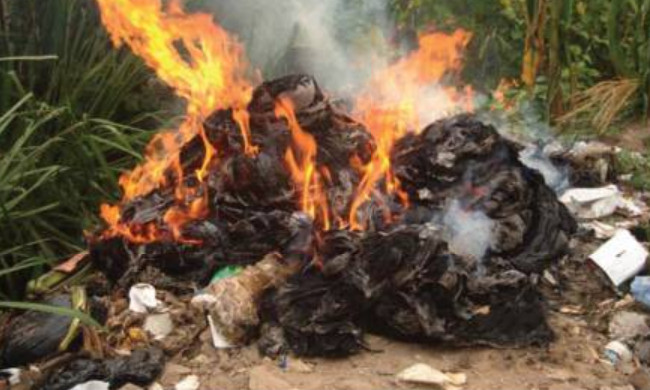
\includegraphics[width=0.5\linewidth]{../inputs/images/zheng/arku3.jpeg}
    \caption{Queima de lixo a céu aberto em Nima. Por Raphael Arku 
           (reprodução autorizada pelo autor).\label{fig:nima_lixo}}
\end{figure} 

Por fim, Acra é mundialmente conhecida por receber ilegalmente lixo 
eletrônico de países industrializados, principalmente europeus, 
que são impropriamente derretidos para a obtenção de cobre pela população local
\citep{asampong2015}. 
O depósito de lixo eletrônico ou \textit{Electronic Waste} (e-waste) está 
localizado no bairro Agbogbloshie, apenas $4 km$ a sudoeste de 
Nima, bairro analisado nesta pesquisa. 
O bromo (Br) compõe plásticos antichama, particularmente em fios, enquanto o 
zinco (Zn) é o principal composto de baterias de eletrônicos. 
Altas concentrações de Al, Co, Cu, Zn, Cd, In, Sb, Ba, e Pb foram encontradas 
no solo do \textit{e-waste} de Agbogbloshie por \citet{asante2012}, 
que também observou altos nível de Fe, Sb, e Pb nas urinas de trabalhadores 
de Agbogbloshie, em contraste com pessoas de referência
(que não tenha tido contato com \textit{e-waste}).

\begin{figure}[H]
  \centering
  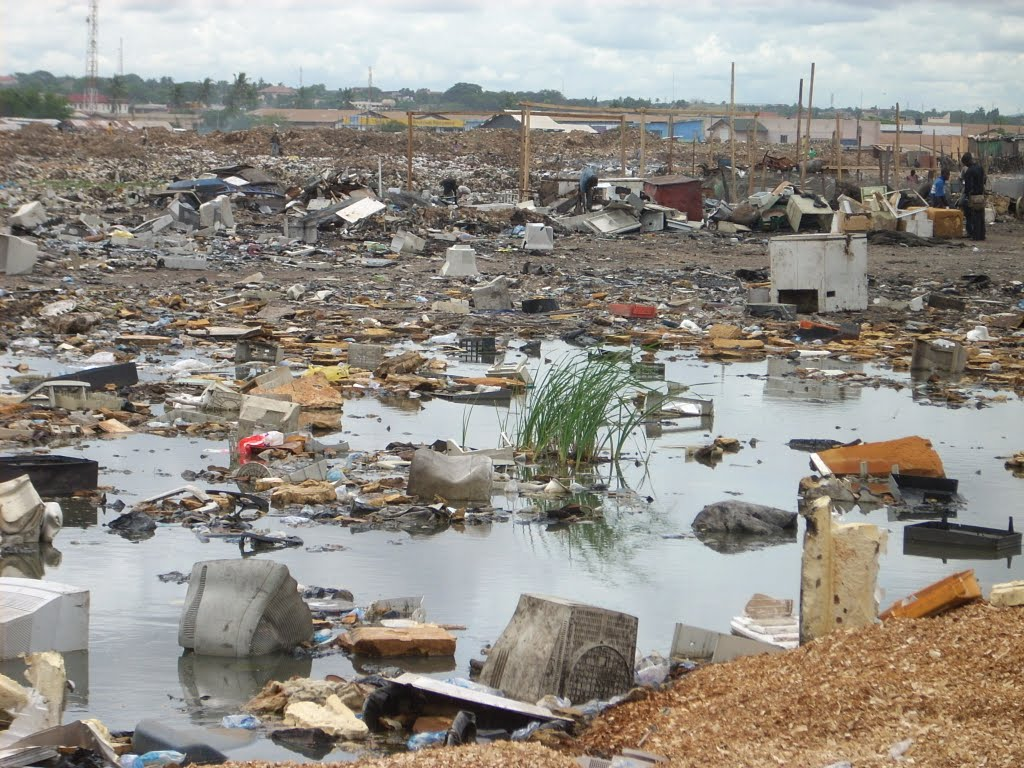
\includegraphics[width=0.5\textwidth]{../inputs/images/ewaste_jack_caravano.jpg}
  \caption{Foto do depósito de lixo eletrônico (e-waste) situado no bairro 
           de Agbogbloshie em Acra. Fotografia de Jack Caravanos, 
           Professor da School of Public Health em Hunter College, CUNY
           Nova Iorque, Estado Unidos da América 
           (reprodução autorizada pelo autor). \label{fig:ewaste}}
\end{figure}

%%%%
%\newpage
\subsection{Nima}

Nima é um dos bairros mais pobres de Acra. É formada de assentamentos não 
planejados, compostos principalmente de migrantes das partes rurais e 
imigrantes de países vizinhos que buscam oportunidades de empregos na capital, 
tornado o bairro diversificado cultural e religiosamente. É conhecido por uma 
feira de comidas típicas permanentemente instalada na região,
\textit{The Nima Market}, que atende a população local e é visitada por turistas que 
transitam por Acra.

Com moradias extremamente improvisadas e vias não pavimentadas, carece de 
sistema de tratamento de esgoto, fornecimento de água potável e eletricidade. 
O meio de transporte dos trabalhadores de Nima para a zona industrial e de 
serviços de Acra é feito por \textit{tro-tro} (vans, no Brasil), podendo ser vistas na foto 
\ref{fig:nima_tro}, que também mostra o congestionamento, característico de 
meios urbanos.  

\begin{figure}[H]
  \centering
    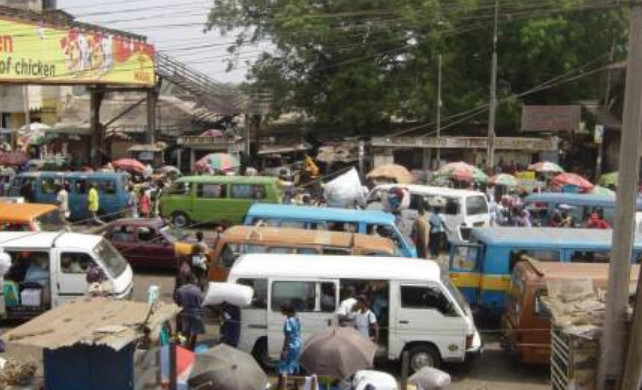
\includegraphics[width=0.5\linewidth]{../inputs/images/zheng/arku4.jpeg}
    \caption{tro-tro e congestionamento em Nima. por Raphael Arku 
           (reprodução autorizada pelo autor). \label{fig:nima_tro}}
\end{figure}

As cozinhas dos moradores de Nima são instalações simples, adaptadas para o uso
de carvão e lenha, podendo ser observadas nas imagens da figura \ref{fig:nima}.

\begin{figure}[H]
  \centering
  \begin{subfigure}[b]{0.4\linewidth}
    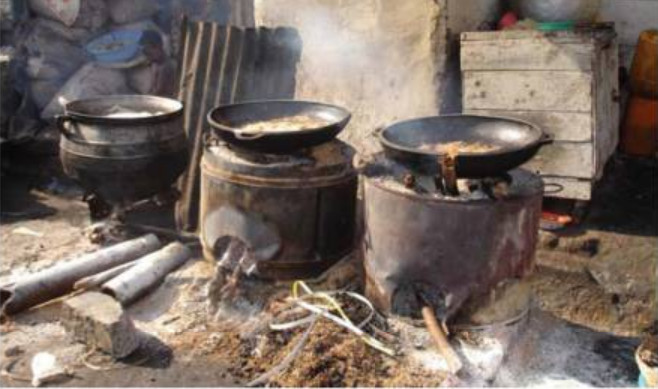
\includegraphics[width=\linewidth]{../inputs/images/zheng/arku1.jpeg}
    \caption{Cozinha residencial em Nima adaptada para o uso de lenha.}
  \end{subfigure}%
  \hspace{0.5cm}
  \begin{subfigure}[b]{0.4\linewidth}
    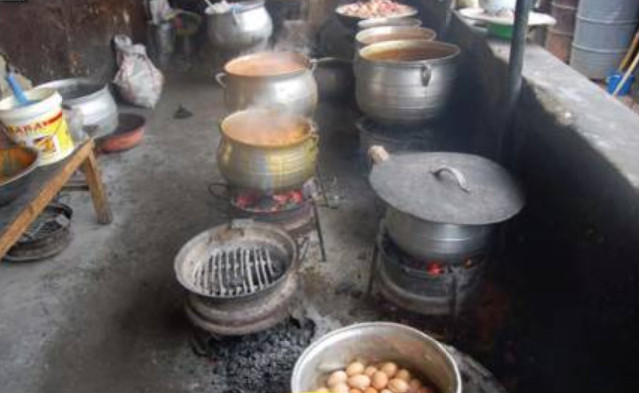
\includegraphics[width=\linewidth]{../inputs/images/zheng/arku2.jpeg}
    \caption{Cozinha de comércio em Nima adaptada para o uso de carvão.}
  \end{subfigure}
  \caption{Fotos de cozinha residencial e comercial de Nima, por Raphael Arku 
           (reprodução autorizada pelo autor). \label{fig:nima}}
\end{figure}
